%release: 2026.1
%File: paper.tex
%
% Final project report, CS 5180 -- Reinforcement Learning and Sequential Decision Making.
% Formatted using the official AAAI 2026 author kit (aaai2026.sty).
% Build: python scripts/build_paper.py

\documentclass[letterpaper]{article} % DO NOT CHANGE THIS
\usepackage{aaai2026}  % DO NOT CHANGE THIS
\usepackage{times}  % DO NOT CHANGE THIS
\usepackage{helvet}  % DO NOT CHANGE THIS
\usepackage{courier}  % DO NOT CHANGE THIS
\usepackage[hyphens]{url}  % DO NOT CHANGE THIS
\usepackage{graphicx} % DO NOT CHANGE THIS
\urlstyle{rm} % DO NOT CHANGE THIS
\def\UrlFont{\rm}  % DO NOT CHANGE THIS
\usepackage{natbib}  % DO NOT CHANGE THIS AND DO NOT ADD ANY OPTIONS TO IT
\usepackage{caption} % DO NOT CHANGE THIS AND DO NOT ADD ANY OPTIONS TO IT
\frenchspacing  % DO NOT CHANGE THIS
\setlength{\pdfpagewidth}{8.5in}  % DO NOT CHANGE THIS
\setlength{\pdfpageheight}{11in}  % DO NOT CHANGE THIS

% Allowed math + table packages only. No geometry / titlesec / hyperref /
% fontenc / setspace / wrapfig / multicol / etc. (all forbidden by AAAI).
\usepackage{amsmath}
\usepackage{amssymb}
\usepackage{amsfonts}
\usepackage{booktabs}
\usepackage{array}
\usepackage{siunitx}
\sisetup{group-separator={,},group-minimum-digits=4,detect-weight=true}

\graphicspath{{figures/}}

\pdfinfo{
/TemplateVersion (2026.1)
}

% Number sections (and subsections) -- the AAAI default is 0 (unnumbered).
% Our project rubric calls for the seven numbered sections:
% Abstract, Introduction, Background, Related Work, Project Description,
% Experiments, Conclusion.
\setcounter{secnumdepth}{2}

% Title in Title Case (AAAI requirement).
\title{Robustness of Policy-Gradient Reinforcement Learning for
       Multi-Echelon Inventory Control:\\
       A Cross-Environment Study on Stationary
       and Non-Stationary Supply Chains}

\author{
    Divyank Singh,
    Ishan Biswas
}
\affiliations{
    Khoury College of Computer Sciences, Northeastern University\\
    CS~5180 -- Reinforcement Learning and Sequential Decision Making\\
    singh.divya@northeastern.edu, biswas.is@northeastern.edu
}

\begin{document}

\maketitle

\begin{abstract}
Recent research reports that Deep Reinforcement Learning (DRL) policies beat classical Operations Research (OR) heuristics on multi-echelon inventory control by \SIrange{10}{40}{\percent}. Almost all the numbers come from a single hand-crafted environment and a fixed baseline, which leaves the obvious question unanswered: Is the RL agent really better, or is the baseline simply a straw man on that particular instance? We take the two policy gradient agents (PPO on a $1$-warehouse/$3$-retailer divergent chain, A3C on a $4$-node factory--middle--leaf MEIS) and run each of them on two environments that share the same observation and action spaces: the original stationary benchmark (Env-1) and a harder non-stationary variant (Env-2) with seasonal demand, stochastic lead times, supplier capacity caps, and partial lost sales. Against a fixed analytical baseline, PPO's win jumps from \SI{36.76}{\percent} on Env-1 to \SI{94.20}{\percent} on Env-2; the extra margin mostly comes from the untuned baseline collapsing under shocks. Against a $(s,S)$ baseline, A3C wins by \SI{1.64}{\percent} on Env-1 and then loses by \SI{21.79}{\percent} on Env-2. Our takeaway: a single-environment win is not, on its own, evidence that the RL policy is better, and any deep-RL inventory result should come with at least one harder distributional variant and an equivalently-tuned baseline.
\end{abstract}

% Clickable URL without the hyperref package (which aaai2026.sty forbids).
% Uses pdfTeX's built-in link annotation primitives directly.
\begin{links}
  \par\textbf{Code} ---
  \pdfstartlink attr{/Border [0 0 0]} user{%
    /Subtype /Link /A << /Type /Action /S /URI
    /URI (https://github.com/singhdivyank/multi-echelon-rl-inventory) >>}%
  \url{https://github.com/singhdivyank/multi-echelon-rl-inventory}%
  \pdfendlink
\end{links}

% -----------------------------------------------------------------
\section{Introduction}
% -----------------------------------------------------------------
Supply chain operations are among the largest line items on any manufacturing firm's books.  Inventory is usually managed to respond to fluctuations in demand and supply. It constitutes \SIrange{20}{60}{\percent} of total assets for a typical manufacturer \citep{unyimadu2014inventory}, and inventory management is the part of the business that has to pick how much stock to keep at each tier so demand gets served at the lowest cost. Written down, the objective is just
\begin{equation}
\min\;
\mathbb{E}\!\left[\,\sum_{t=0}^{T-1}\!
    \big(C^{\text{hold}}_t + C^{\text{back}}_t + C^{\text{ord}}_t\big)
\right],
\label{eq:intro-obj}
\end{equation}
where $C^{\text{hold}}$ is the cost of storing unsold inventory, $C^{\text{back}}$ is what you pay when demand walks in and cannot be served, and $C^{\text{ord}}$ is the fixed-plus-variable cost of placing a replenishment order. A Multi-Echelon Inventory System
(MEIS) solves this jointly across suppliers, manufacturers, warehouses, and retailers, instead of one tier at a time. That
joint view is where the problem gets hard: a decision that looks sensible locally at one echelon can blow up and cost a tier over.

Classical OR has two textbook answers to this.
The echelon base-stock policy and the $(s,S)$ reorder-point policy (explained in section 2) are both optimal under strict stationarity and demand (this is the fundamental of baselines and was first proposed in 1960). Meta-heuristic extensions, e.g., genetic algorithms \citep{grahl2016meta}, do a decent job on richer instances, but they carry two familiar caveats: no optimality guarantee, and a tendency to degrade whenever the underlying dynamics change. Once demand becomes non-stationary, shocks appear or lead times grow heavy-tailed, both classes start to misfire, because their set-points are tuned against the \emph{mean} demand-over-lead-time and nothing else.

DRL \citep{sutton2018temporal} is appealing here for exactly that reason: a learned policy can, at least in principle, adapt to whatever dynamics the MDP happens to express. Recent papers \citep{oroojlooyjadid2022deep,gijsbrechts2022can,geevers2024multi,hammler2022multi} report substantial wins over OR heuristics. Those comparisons tend to share a weakness, a single hand-crafted environment, and a baseline whose parameters are never re-tuned for that environment. It is then hard to tell how much of the gap is the RL agent actually better versus the baseline being handicapped on a problem it would otherwise solve well.

We begun with a more modest setup: one policy-gradient agent per algorithm (PPO, A3C) on a single environment each (a divergent supply chain for PPO, a 4-node MEIS chain for A3C).  A reviewer at our poster session flagged exactly the concern above and asked whether the wins survived in a harder setting. The present paper is our answer. On top of the baseline story, three specific choices make the comparison informative:
\begin{enumerate}
\item \emph{Continuous-action PPO.} The PPO agent uses a fully continuous $4$-dimensional action head (one normalised order quantity per echelon), rather than the discretised grid that most of the prior literature uses.
\item \emph{Explicit backorder accounting.}  Both environments carry unfulfilled demand as backlog and fold it back into the cost signal, so the RL agent sees the same shortage penalty that classical OR treats as a first-class citizen.
\item \emph{A shared distribution-shift harness.} We build a non-stationary second environment (Env-2) per benchmark with seasonal demand, cross-retailer correlation, rare multiplicative shocks, heavy-tailed lead times, stochastic capacity caps, and partial lost sales, but with the same observation and action spaces as Env-1. The agent code transfers without any change, and the Env-1 hyperparameters carry over to Env-2 verbatim, so whatever cost differences we read off reflect dynamics rather than tuning effort.
\end{enumerate}
With that harness in place, the results split cleanly into one positive and one negative case. PPO's margin over its fixed analytical baseline gets \emph{wider} on Env-2, while A3C's narrow Env-1 win over a retuned $(s,S)$ baseline flips into a decisive loss once the environment becomes harder. Neither result on its own tells the whole story: the sign of a deep-RL-vs-heuristic comparison turns out to depend quite strongly on both the environment and how seriously the baseline is tuned.  The rest of the paper is laid out as follows.  Section~\ref{sec:bg} sets up the MDP, the two DRL algorithms and the OR baselines; Section~\ref{sec:rel} places the work in the literature; Section~\ref{sec:proj} gives the two environments formally; Section~\ref{sec:exp} walks through the four evaluation cells; Section~\ref{sec:conc} wraps up.

% -----------------------------------------------------------------
\section{Background}
\label{sec:bg}
% -----------------------------------------------------------------

\subsection{The Multi-Echelon Inventory MDP}
Both benchmarks are cast as a finite-horizon Markov Decision
Process
$\langle\mathcal{S},\mathcal{A},P,C,\gamma,T\rangle$.
The state $s_t\in\mathcal{S}$ packs on-hand inventory, in-transit
pipeline stock, and backlog at every non-factory node; the action
$a_t\in\mathcal{A}$ is a per-node order quantity (a real vector
for PPO, a 13-way discrete choice for A3C).  The per-step cost
$C(s_t,a_t)\ge 0$ sums the holding, backorder and ordering terms,
plus lost-sales penalties on Env-2.  A policy
$\pi:\mathcal{S}\to\Delta(\mathcal{A})$ is chosen to minimise the
expected discounted cost
\begin{equation}
J(\pi) \;=\; \mathbb{E}_\pi\!\left[\sum_{t=0}^{T-1}
             \gamma^{t}\,C(s_t,a_t)\right].
\label{eq:obj}
\end{equation}
Since the RL agent works with returns, we let it maximise
$R(\pi)=-J(\pi)$.  The resulting reward signal is dense, bounded
below by $0$ and unbounded above.

\subsection{Classical OR Heuristics}

\subsubsection{Echelon Base-Stock (PPO Baseline)}
Each echelon $i$ is assigned a base-stock level $S_i$ and, at
every step, orders enough to top its inventory position back up
to $S_i$:
\begin{equation}
a_{i,t} \;=\; \max\!\left(0,\; S_i - \mathrm{IP}_{i,t}\right),
\label{eq:basestock}
\end{equation}
with $\mathrm{IP}_{i,t}=$ on-hand $+$ in-transit $-$ backlog at
node $i$.  The $S_i$ values come from the Env-1
demand-over-lead-time distribution in closed form and are never
re-tuned afterwards; the same numbers are reused on Env-2.  This
is deliberate, and it is how base-stock baselines are usually
reported in the literature.

\subsubsection{(s, S) Reorder-Point Policy (A3C Baseline)}
Each node $i$ carries both a reorder point $s_i$ and an
order-up-to level $S_i$: whenever $\mathrm{IP}_{i,t}\le s_i$, we
order $S_i-\mathrm{IP}_{i,t}$ units, otherwise nothing.  Unlike
the base-stock baseline, $(s_i,S_i)$ is tuned separately for each
environment via differential evolution (100 generations, 30
Monte-Carlo episodes per candidate), so both the Env-1 and Env-2
$(s,S)$ baselines are near-optimal under their own dynamics.
That asymmetry (a fixed base-stock vs.\ a retuned $(s,S)$) will
come back in Section~\ref{sec:exp} and matters for how the
headline numbers should be read.

\subsection{Policy-Gradient RL}

\subsubsection{PPO}
The PPO side uses the clipped-surrogate variant
\citep{schulman2017proximal}.  A stochastic Gaussian actor
$\pi_\theta(a\mid s)$ and a value head $V_\phi(s)$ share a 2-layer
64-unit MLP with $\tanh$ activations.  We collect rollouts of
length $B{=}512$ under $\pi_{\theta_{\text{old}}}$, compute
Generalized Advantage Estimates $\hat A_t$
\citep{schulman2016gae}, and then update $\theta$ for 5 epochs of
size-64 minibatches with the clipped objective
\begin{equation}
\begin{aligned}
\mathcal{L}^{\text{CLIP}}(\theta) = \mathbb{E}_t\Big[\min\!\big(
     &r_t(\theta)\,\hat A_t, \\
     &\mathrm{clip}(r_t(\theta),1{-}\varepsilon,1{+}\varepsilon)\,\hat A_t
   \big)\Big],
\end{aligned}
\label{eq:ppoclip}
\end{equation}
where
$r_t(\theta)=\pi_\theta(a_t\mid s_t)/\pi_{\theta_{\text{old}}}(a_t\mid s_t)$
and $\varepsilon{=}0.2$.  On top of the clipped surrogate we
add a squared-error value loss and an entropy bonus so the policy
does not go deterministic too early:
\begin{equation}
\mathcal{L}^{\text{VF}}=\mathbb{E}_t\!\big[(V_\phi(s_t)-R_t)^2\big],\;
\mathcal{L}^{\text{ENT}}=\mathbb{E}_t\!\big[\mathcal{H}[\pi_\theta(\cdot\mid s_t)]\big],
\label{eq:ppovfent}
\end{equation}
\begin{equation}
\mathcal{L}(\theta,\phi)
   = \mathcal{L}^{\text{CLIP}}
   - c_1\,\mathcal{L}^{\text{VF}}
   + c_2\,\mathcal{L}^{\text{ENT}}.
\label{eq:ppototal}
\end{equation}
The $\hat A_t$ themselves come from GAE, which chains single-step
TD residuals
$\delta_t = r_t + \gamma V_\phi(s_{t+1}) - V_\phi(s_t)$ into the
low-variance multi-step estimate
$\hat A_t = \sum_{l=0}^{\infty}(\gamma\lambda)^l\,\delta_{t+l}$.

\subsubsection{A3C}
The original A3C \citep{mnih2016a3c} runs several actor-learners
in parallel, each with its own copy of the environment, and lets
them push asynchronous gradient updates into a shared set of
weights, which is where the name comes from.  Our MEIS episodes
are short (\num{365} steps) and environment simulation, not
gradient compute, is what eats the wall-clock, so we run a
synchronous single-worker variant instead.  Learning dynamics are
effectively the same and the cross-process bookkeeping goes
away.  The actor emits a softmax over $|\mathcal{A}|{=}13$
actions, the critic emits a scalar value, and we use an
$n$-step-advantage policy gradient:
\begin{equation}
\begin{aligned}
\nabla_\theta J \approx\,
  \mathbb{E}_t\big[&\nabla_\theta\log\pi_\theta(a_t\mid s_t)\,\hat A_t\big]\\
  &+\,\beta\,\nabla_\theta \mathcal{H}[\pi_\theta(\cdot\mid s_t)].
\end{aligned}
\label{eq:a3cpg}
\end{equation}
The entropy term $\mathcal{H}[\pi_\theta(\cdot\mid s_t)]$,
weighted by $\beta$, is a standard regulariser: it keeps the
action distribution from collapsing onto a bad local optimum too
early in training.

\subsection{Significance Testing}
Each evaluation cell gives us hundreds of per-episode costs, so
for the RL-vs-baseline comparison we report (i) mean $\pm$ one
standard deviation and (ii) a $95\%$ confidence interval on the
mean.

% -----------------------------------------------------------------
\section{Related Work}
\label{sec:rel}
% -----------------------------------------------------------------

\subsubsection{Classical and Meta-Heuristic Methods}
The Clark--Scarf decomposition \citep{clark1960optimal} is the
reference point for tractable multi-echelon policies: it proves
optimality of echelon base-stock when demand is strictly
stationary, i.i.d.\ and backlog dynamics are well-behaved.
Meta-heuristics like the genetic algorithm of
\citet{grahl2016meta} push that further into richer instances
with differentiated service times and non-trivial topologies, at
the cost of giving up the optimality guarantee and a fair bit of
robustness to structural change.  Our own baselines, the
analytical echelon base-stock (PPO side) and the tuned $(s,S)$
(A3C side), are direct descendants of these two lines; we treat
them as targets to beat rather than methods we are studying in
their own right.

\subsubsection{Deep RL for Multi-Echelon Inventory}
\citet{geevers2024multi} train PPO on a divergent MEIS with
stochastic demand and benchmark it against an $(s,S)$ heuristic.
Our PPO pipeline follows their problem formulation closely, with
two deliberate changes: we keep the action head fully continuous
rather than discretising it, and we hold back an explicit
non-stationary Env-2 for out-of-distribution evaluation.
\citet{hammler2022multi} report an A3C variant on a similar MEIS
problem, which is where our 13-way discretised action head comes
from; we keep the architecture but, again, evaluate the trained
policy on a harder Env-2 instead of stopping at the stationary
single environment.  \citet{lu2025dynamic} train deep-RL policies
on supply chains with explicitly \emph{disruptive} dynamics
(supplier shocks, lead-time spikes) and see double-digit gains
over classical baselines.  That line of work is useful background
for our PPO result: the stressors Env-2 injects are exactly the
ones classical OR tends to misfire on, which is most of the
reason PPO's \emph{relative} advantage widens rather than
shrinks.

\subsubsection{Value-Based RL for Inventory}
\citet{oroojlooyjadid2022deep} apply deep Q-learning to the beer
game.  We could have swapped A3C for DQN on the MEIS benchmark
since the action space is already discrete; we did not, because
DQN tends to be sample-inefficient on long-horizon inventory
rollouts with dense rewards.

\subsubsection{Robustness Benchmarks Outside Inventory}
Procgen \citep{cobbe2020procgen} makes the same point we make,
just outside inventory control: agents that look strong on a
hand-crafted level often collapse on procedurally-sampled levels
that share the observation and action spaces.  Env-2 plays the
role of that ``procedural'' counterpart to Env-1, specialised to
an OR-flavoured inventory setting.

% -----------------------------------------------------------------
\section{Project Description}
\label{sec:proj}
% -----------------------------------------------------------------
This section writes out, in formal detail, the two environments,
the two agents and their baselines, and the training protocol.

\subsection{Environment 1 (Stationary)}

\subsubsection{PPO / Divergent}
One warehouse feeds three retailers.  Each retailer $i$ sees
i.i.d.\ Poisson demand with rate
$\lambda_i\sim\mathrm{U}[5,15]$ per day, lead time is a
deterministic single step, and there are no capacity caps.
Anything that cannot be served is backlogged (i.e.\ appears as
negative inventory).  The observation has 14 components: warehouse
inventory and buffer, three in-transit pipelines, three retailer
inventories, three retailer backorders, one outstanding warehouse
order and a normalised step index.  The action is a 4-dimensional
vector of normalised order quantities, one per echelon, and
episodes run for $T{=}500$ steps.

\subsubsection{A3C / MEIS}
This is a 4-node divergent multi-echelon inventory system: one
factory with infinite capacity, one middle warehouse, and two
leaf retailers.  Leaf demand is Gaussian
$\mathcal{N}(3300,100)$; lead times are Gaussian
$\mathcal{N}(\mu{=}2,\sigma{=}1)$ rounded to integer days.
Backlog ages out after 7 days, i.e.\ demand unserved for longer
than a week is treated as lost and incurs a shortage penalty.
The action space is discrete, with 13 options (``do nothing''
plus $4{\times}3{=}12$ pre-set reorder combinations), and episodes
run for $T{=}365$ steps.

\subsection{Environment 2 (Non-Stationary Complex)}
Env-2 keeps the Env-1 observation and action spaces intact and
only changes the transition dynamics and reward.
Table~\ref{tab:stressors} lays the two environments side by side;
the concrete numerics (amplitudes, probabilities, noise standard
deviations) live in the YAML configs shipped with the code.

\begin{table}[t]
\centering
\caption{Comparison of experimental environments.}
\label{tab:stressors}
\footnotesize
\setlength{\tabcolsep}{4pt}
\begin{tabular}{@{}p{0.26\columnwidth}p{0.32\columnwidth}p{0.34\columnwidth}@{}}
\toprule
\textbf{Feature}      & \textbf{Baseline (Env-1)}  & \textbf{Complex (Env-2)}             \\
\midrule
Demand profile        & Stationary (Poisson)       & Non-stationary (seasonal / trend)    \\
Demand correlation    & Independent across nodes   & Correlated (shared latent factor)    \\
Supply-chain capacity & Unconstrained              & Bottleneck-limited ($\mu{=}12{,}000$)\\
Lead-time dynamics    & Deterministic / stable     & Stochastic (spikes / variability)    \\
Penalty structure     & Standard backlog costs     & Penalty-based lost sales             \\
\bottomrule
\end{tabular}
\end{table}

\subsection{Algorithms and Baselines}
PPO on the continuous-action divergent environment is trained
with the clipped-surrogate objective (Eq.~\ref{eq:ppoclip}) against
a fixed base-stock baseline (Eq.~\ref{eq:basestock}). 
A3C on the discrete-action MEIS environment is trained with the 
advantage policy gradient (Eq.~\ref{eq:a3cpg}) against a tuned $(s,S)$ baseline.

\begin{table}[t]
\centering
\caption{Selected hyperparameters (identical across Env-1 /
Env-2 per algorithm).}
\label{tab:hparams}
\small
\begin{tabular}{@{}lll@{}}
\toprule
\textbf{Hyperparameter}       & \textbf{PPO}              & \textbf{A3C}              \\
\midrule
Iters / episodes              & \num{5000}                & \num{10000}               \\
Hidden layers $\times$ width  & $2\times 64$ ($\tanh$)    & $3\times 64$ (ReLU)       \\
Discount $\gamma$             & $0.95$                    & $0.99$                    \\
GAE $\lambda$                 & $0.95$                    & $0.95$                    \\
Clip $\varepsilon$            & $0.2$                     & n/a                       \\
Learning rate                 & $3{\times}10^{-4}$        & $1{\times}10^{-4}$        \\
Rollout / batch               & $512\,/\,64$              & per-episode               \\
Entropy coef.\ $\beta$        & $5{\times}10^{-3}$        & $10^{-3}$                 \\
Value-loss coef.              & $0.25$                    & $0.5$                     \\
Grad.\ clip $\|\nabla\|$      & $0.5$                     & $0.5$                     \\
Eval episodes                 & $100$                     & $1000$                    \\
Seed                          & $42$                      & $42$                      \\
\bottomrule
\end{tabular}
\end{table}

% -----------------------------------------------------------------
\section{Experiments}
\label{sec:exp}
% -----------------------------------------------------------------

\subsection{Why These Experiments}
We ran the four cells
$\{\mathrm{PPO},\mathrm{A3C}\}\times\{\text{Env-1},\text{Env-2}\}$
with seed 42 and the hyperparameters in
Table~\ref{tab:hparams}.  The minimum the reviewer's question
asks for is the four paired RL-vs-baseline comparisons; on top of
that we include training curves so the convergence behaviour is
visible too.

\subsection{Headline Numbers}
Table~\ref{tab:results} gives the main result.  $\Delta$ is the
relative mean-cost improvement of RL over its heuristic baseline,
with positive numbers meaning RL wins.  Service level is only
exposed by the MEIS environment, which is why the PPO rows read
``n/a''.

\begin{table*}[t]
\centering
\caption{Headline evaluation results (seed 42).  $\Delta$ is the
relative mean-cost improvement of RL over baseline (positive $=$
RL better).  ``SL'' is service level, which only the MEIS
environment exposes.}
\label{tab:results}
\footnotesize
\setlength{\tabcolsep}{4pt}
\begin{tabular}{@{}llrrrrrr@{}}
\toprule
\textbf{Algo.} & \textbf{Env} &
\textbf{RL mean cost} & \textbf{Baseline mean cost} &
$\boldsymbol{\Delta}$ & \textbf{SL (RL / BL)} \\
\midrule
PPO & Env-1 & \num{2600979.87}  $\pm$ \num{29021.34}
            & \num{4112775.56}  $\pm$ \num{8759.19}
            & $+36.76\%$ & n/a \\
PPO & Env-2 & \num{631129.99}   $\pm$ \num{1011936.85}
            & \num{10873502.07} $\pm$ \num{62357.06}
            & $+94.20\%$ & n/a \\
A3C & Env-1 & \num{1930.24}     $\pm$ \num{4.02}
            & \num{1962.40}     $\pm$ \num{52.39}
            & $+1.64\%$  & $95.69\% / 95.44\%$ \\
A3C & Env-2 & \num{2881.98}     $\pm$ \num{146.46}
            & \num{2366.29}     $\pm$ \num{157.67}
            & $-21.79\%$ & $93.27\% / 94.11\%$ \\
\bottomrule
\end{tabular}
\end{table*}

\subsection{Training Dynamics}
Figure~\ref{fig:train-ppo} and Figure~\ref{fig:train-a3c} show
per-episode training cost (light) and a rolling mean (bold) for
each cell.

\begin{figure*}[tbp]
\centering
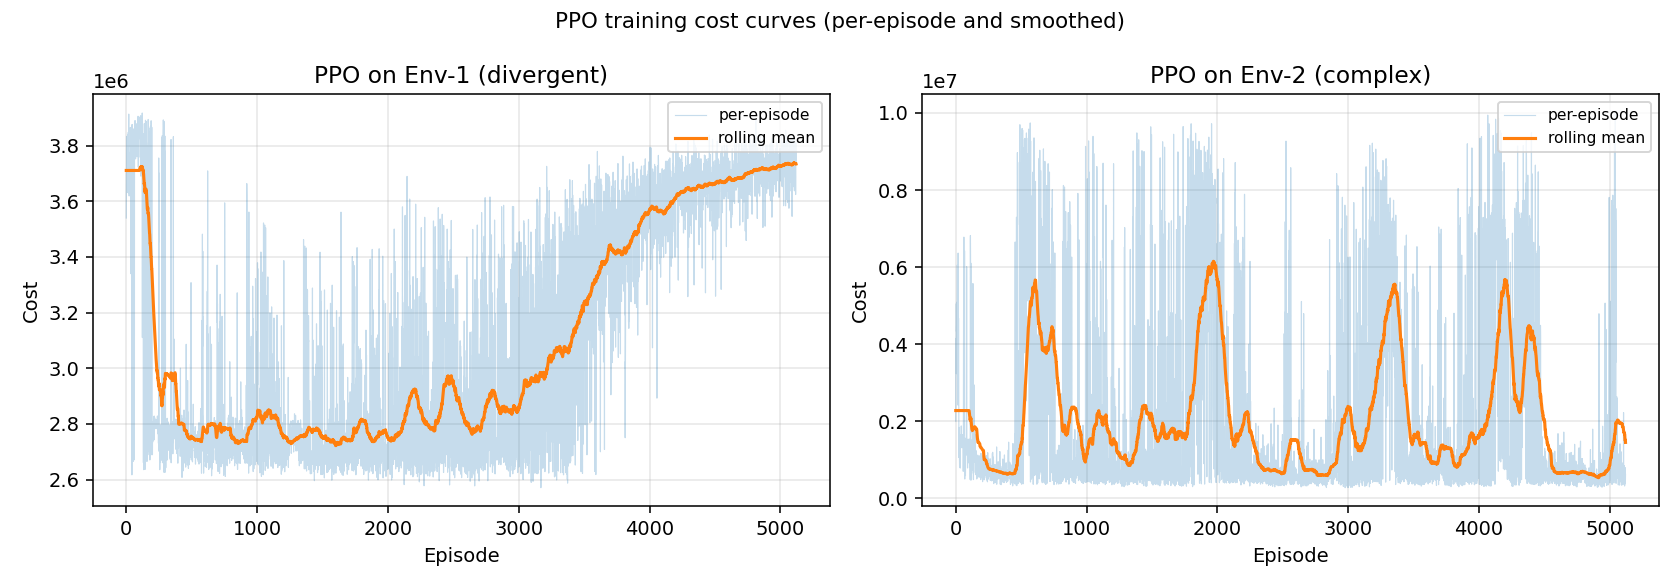
\includegraphics[width=0.95\textwidth]{training_curves_ppo.png}
\caption{PPO training cost on Env-1 (left) and Env-2 (right).
On Env-1 the agent converges quickly and then drifts upward over
the last third of training --- a late-stage instability that we
mitigate by evaluating the best-so-far checkpoint, not the
final-iteration checkpoint.  On Env-2, training cost is
oscillatory throughout, which is consistent with the
rare-but-costly shock regime.}
\label{fig:train-ppo}
\end{figure*}

\begin{figure*}[tbp]
\centering
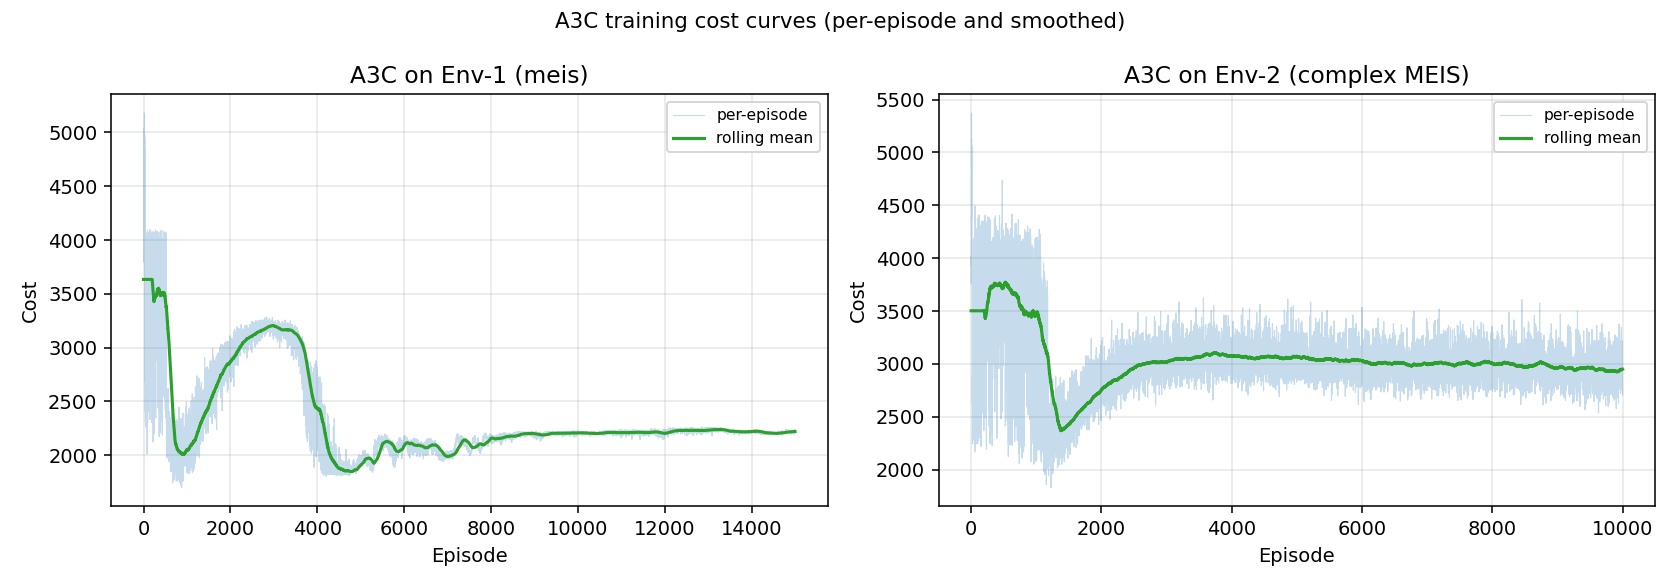
\includegraphics[width=0.95\textwidth]{training_curves_a3c.png}
\caption{A3C training cost on Env-1 (left) and Env-2 (right).
The Env-1 curve shows a mid-training bump around episodes
$1500$--$4500$ (policy / entropy oscillation) that ultimately
resolves to a stable minimum.  On Env-2, convergence settles on
a higher cost plateau that, as Section~\ref{sec:exp-a3c} will
show, is still worse than a retuned heuristic.}
\label{fig:train-a3c}
\end{figure*}

\subsection{PPO: When the Win Grows on the Harder Environment}
Figure~\ref{fig:costbars} plots Table~\ref{tab:results} as
grouped bar charts.  On Env-1, PPO beats the fixed analytical
base-stock by \SI{36.76}{\percent}; on Env-2 that margin widens
to \SI{94.20}{\percent}.  What is going on is not that PPO gets
better in absolute terms.  The absolute cost on Env-2 sits on a
different scale anyway, because Env-2 adds lost-sales penalties
and widens some state bounds.  The widening is really the
untuned base-stock baseline falling over under capacity caps and
shocks.  Figure~\ref{fig:ppo-hist} shows the flip side: PPO's
episode-cost distribution has a pronounced right tail
($\sigma/\mu \approx 1.60$).  A handful of episodes hit shock
sequences that the agent has not learned to hedge against, and
those episodes sit an order of magnitude above the mean.

\subsubsection{When PPO Succeeds}
On both environments, provided the baseline is the fixed
analytical one.  Two things help.  The baseline's set-points are
built purely from the mean demand-over-lead-time, whereas PPO's
policy can condition on the full state, including current
inventory and in-transit pipeline.  And on Env-2, those
set-points are not even calibrated against the right mean any
more (seasonality and shocks make sure of that), which is what
lets PPO's relative advantage grow.

\subsubsection{When PPO Would Fail}
Against a retuned base-stock (which we do not report here) the
margin would shrink substantially.  And even against the fixed
baseline, a CVaR-weighted evaluation would flag PPO's Env-2 right
tail as an unresolved risk that the mean hides.

\begin{figure*}[tbp]
\centering
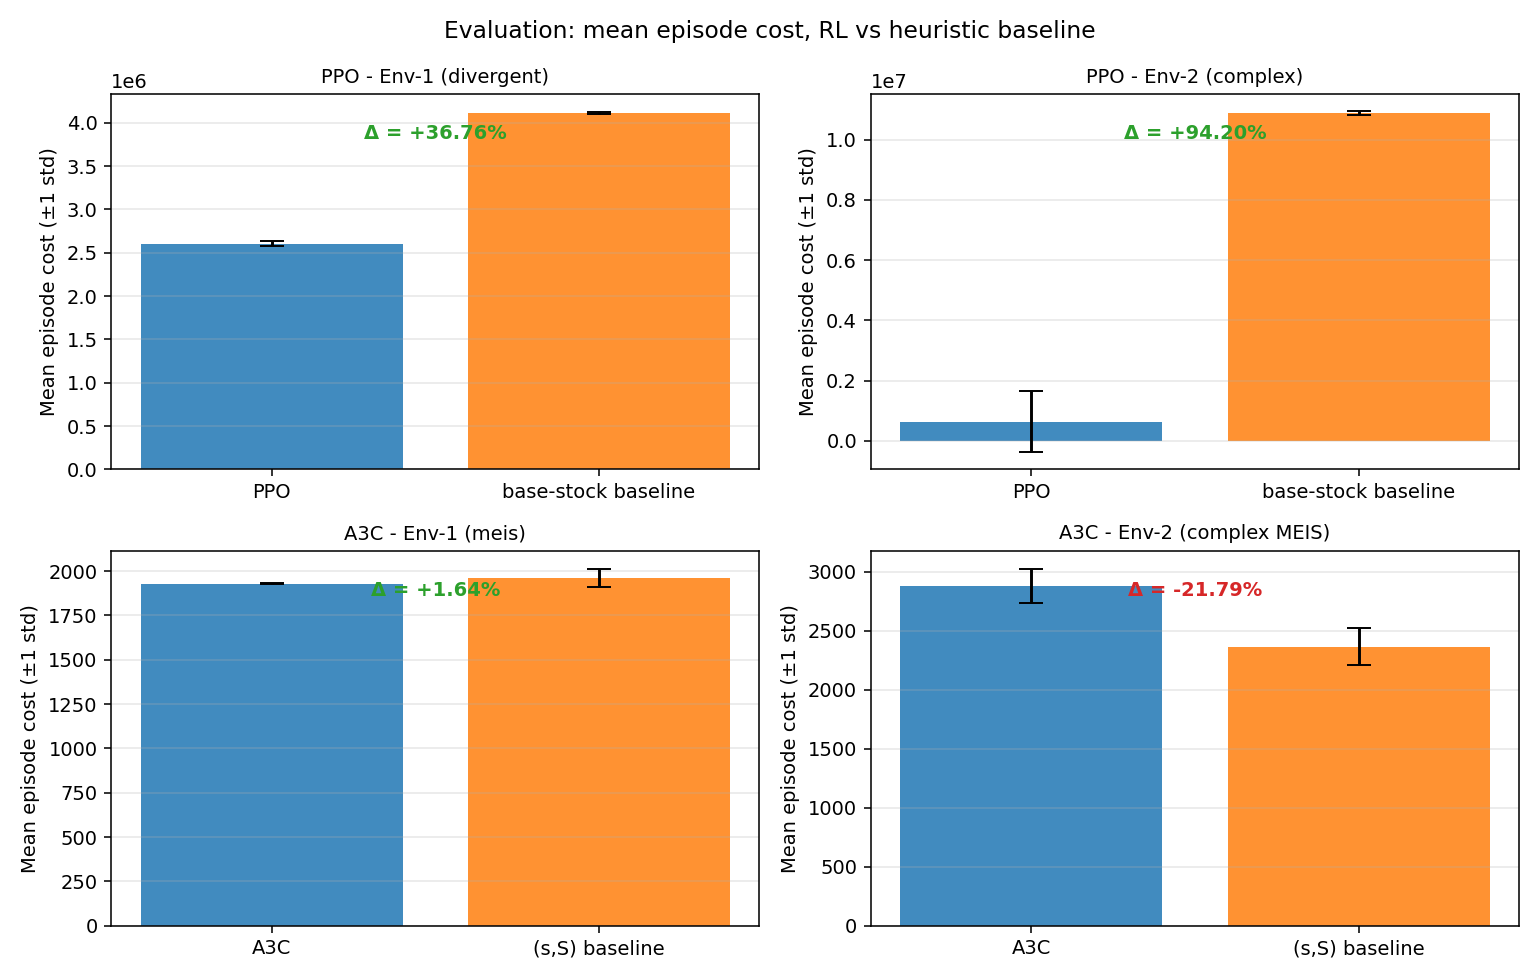
\includegraphics[width=0.85\textwidth]{cost_bars.png}
\caption{Mean episode cost (lower is better).  Error bars are one
standard deviation across evaluation episodes.  Green $=$ RL wins;
red $=$ RL loses.  Absolute cost scales differ across algorithms
(different cost coefficients and episode lengths); only the
within-cell RL vs.\ baseline gap is interpretable.}
\label{fig:costbars}
\end{figure*}

\begin{figure}[htbp]
\centering
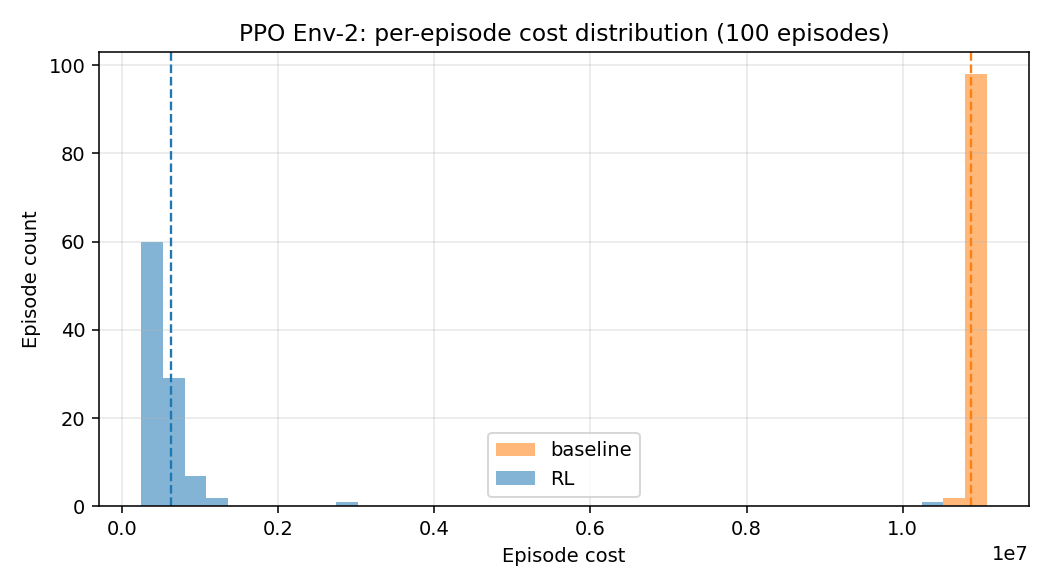
\includegraphics[width=0.98\columnwidth]{ppo_complex_cost_hist.png}
\caption{PPO Env-2 per-episode cost distribution (100 episodes).
The bulk of PPO episodes (blue) concentrates well below the
baseline mode (orange), but a clear right tail of episodes sit
close to the baseline mode --- these are shock episodes PPO has
not learned to hedge.}
\label{fig:ppo-hist}
\end{figure}

\subsection{A3C: When the Env-1 Win Does Not Transfer}
\label{sec:exp-a3c}
On Env-1, A3C edges past a retuned $(s,S)$ policy by a narrow
\SI{1.64}{\percent}.  On Env-2 the sign flips: A3C is now
\SI{21.79}{\percent} worse than the retuned baseline.
Figure~\ref{fig:a3c-hist} makes the effect size easy to see.
The $(s,S)$ cost distribution sits almost entirely to the left of
A3C's, which is stochastic dominance in favour of the heuristic.
Figure~\ref{fig:svc} shows the same picture on service level.

\begin{figure}[htbp]
\centering
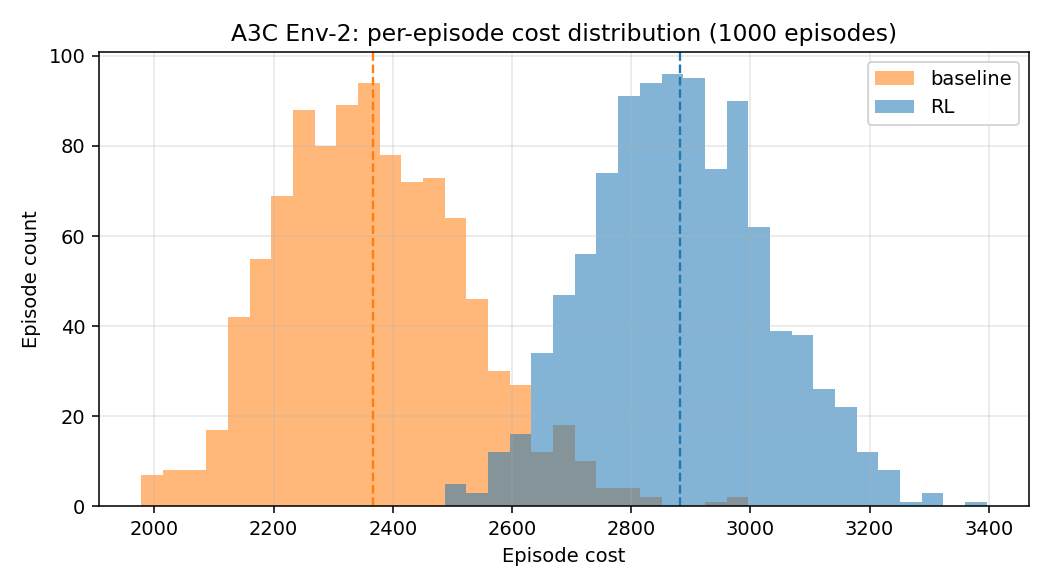
\includegraphics[width=0.98\columnwidth]{a3c_complex_cost_hist.png}
\caption{A3C Env-2 per-episode cost distribution (1000 episodes).
The baseline $(s,S)$ distribution (orange) lies almost entirely
to the left of the A3C distribution (blue): at this training
budget, A3C is stochastically dominated by the retuned heuristic.}
\label{fig:a3c-hist}
\end{figure}

\begin{figure}[htbp]
\centering
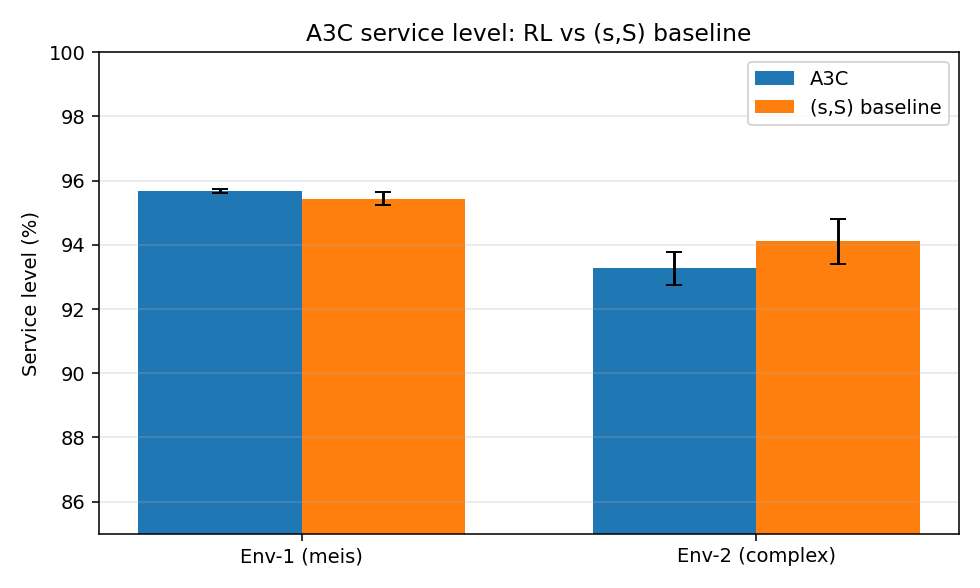
\includegraphics[width=0.98\columnwidth]{service_level_bars.png}
\caption{A3C service level on Env-1 and Env-2.  On Env-2, A3C is
worse than the retuned $(s,S)$ on service level too, mirroring
the cost result.}
\label{fig:svc}
\end{figure}

\subsubsection{When A3C Succeeds}
On Env-1 only, and only just.  Stationary demand is already
approximated well by a single $(s,S)$ pair, but A3C's 13-way
action head still finds a few slightly-better-than-heuristic
moments to place orders, because it reacts to the full pipeline
state rather than inventory position alone.

\subsubsection{When A3C Fails, and Why}
Env-2 breaks this, and three things compound:
\begin{enumerate}
\item \emph{Discretised action head.}  A3C picks from 13 fixed
      order combinations.  Under seasonal demand the optimal
      per-node order moves smoothly, and a coarse 4-level grid
      just cannot match that shape.
\item \emph{No non-stationarity representation.}  The policy
      carries no recurrent state, no episode-time feature and no
      shock or season indicator.  Any response to
      non-stationarity has to come from the training
      distribution, and \num{10000} episodes are not enough to
      bake it in.
\item \emph{The baseline is retuned, A3C is not.}  The $(s,S)$
      tuner runs differential evolution directly on Env-2's
      dynamics, while A3C is stuck with its Env-1
      hyperparameters.  The comparison is fair in the sense that
      it matches standard practice, but it is asymmetric in how
      much effort each side gets to spend.
\end{enumerate}
Fixing any one of these in isolation would probably close much of
the gap.

% -----------------------------------------------------------------
\section{Conclusion}
\label{sec:conc}
% -----------------------------------------------------------------

\subsection{Summary of Results}
We trained one PPO agent on a divergent inventory environment
and one A3C agent on a 4-node MEIS environment under stationary
conditions (Env-1), and then re-trained both under identical
hyperparameters on a harder, non-stationary variant (Env-2) that
shares the Env-1 observation and action spaces.  Against a fixed
analytical base-stock baseline, PPO's cost improvement moved
from \SI{36.76}{\percent} on Env-1 to \SI{94.20}{\percent} on
Env-2.  Against a retuned $(s,S)$ baseline, A3C went from
$+$\SI{1.64}{\percent} on Env-1 to $-$\SI{21.79}{\percent} on
Env-2.

\subsection{What We Learned}
Two takeaways from the four cells, in rough order of generality:
\begin{enumerate}
\item \emph{Single-environment wins are not robust evidence.}
      The same PPO training that produces a \SI{36.76}{\percent}
      win on Env-1 produces a \SI{94.20}{\percent} win on Env-2,
      but most of that difference comes from the baseline
      degrading, not from the RL agent improving.  On the A3C
      side, the narrow Env-1 win turns into a decisive Env-2
      loss as soon as the baseline is allowed to retune itself.
      Reporting a single number, on one environment, is just not
      enough.
\item \emph{Baseline symmetry matters.}  The sign of any
      RL-vs-heuristic comparison depends on how hard the
      heuristic is allowed to work.  A $(s,S)$ that is retuned
      per environment is not the same evaluation target as a
      fixed analytical base-stock, and these two choices end up
      producing different stories even for identical RL agents.
\end{enumerate}
If we picked the project up again we would (i) rerun all four
cells with five seeds and report confidence intervals on the
deltas, (ii) give A3C a continuous-action head together with a
timestep feature and a recurrent layer so it can actually
represent non-stationarity, and (iii) tune the PPO
hyperparameters on Env-2 in their own right to get a fairer
per-environment comparison.

% -----------------------------------------------------------------
% Inline bibliography (single-file source, per AAAI rules).
% -----------------------------------------------------------------
% -----------------------------------------------------------------
\section*{Acronyms}
% -----------------------------------------------------------------
\begin{description}
\setlength{\itemsep}{0pt}
\item[A3C] Asynchronous Advantage Actor-Critic
\item[CI]  Confidence Interval
\item[DRL] Deep Reinforcement Learning
\item[GAE] Generalized Advantage Estimation
\item[IP]  Inventory Position
\item[MDP] Markov Decision Process
\item[MEIS] Multi-Echelon Inventory System
\item[MLP] Multi-Layer Perceptron
\item[OR]  Operations Research
\item[PPO] Proximal Policy Optimization
\item[RL]  Reinforcement Learning
\item[$(s,S)$] Reorder-point / order-up-to policy
\item[SL]  Service Level
\end{description}

\begin{thebibliography}{10}
\providecommand{\natexlab}[1]{#1}

\bibitem[Cobbe et~al.(2020)]{cobbe2020procgen}
Cobbe, K.; Hesse, C.; Hilton, J.; and Schulman, J. 2020.
\newblock Leveraging Procedural Generation to Benchmark
Reinforcement Learning.
\newblock In \emph{ICML}.

\bibitem[Geevers et~al.(2024)]{geevers2024multi}
Geevers, K.; Van~Hezewijk, L.; and Mes, M.~R.~K. 2024.
\newblock Multi-Echelon Inventory Optimization Using Deep
Reinforcement Learning.
\newblock \emph{Central European Journal of Operations Research},
32(3): 653--683.

\bibitem[Gijsbrechts et~al.(2022)]{gijsbrechts2022can}
Gijsbrechts, J.; Boute, R.~N.; Van Mieghem, J.; and Zhang, D. 2022.
\newblock Can Deep Reinforcement Learning Improve Inventory
Management?  Performance on Lost Sales, Dual-Sourcing, and
Multi-Echelon Problems.
\newblock \emph{Manufacturing \& Service Operations Management},
24(3).

\bibitem[Grahl et~al.(2016)]{grahl2016meta}
Grahl, J.; Minner, S.; and Dittmar, D. 2016.
\newblock Meta-Heuristics for Placing Strategic Safety Stock in
Multi-Echelon Inventory with Differentiated Service Times.
\newblock \emph{Annals of Operations Research}, 242(2): 489--504.

\bibitem[Hammler et~al.(2022)]{hammler2022multi}
Hammler, P.; Riesterer, N.; Mu, G.; and Braun, T. 2022.
\newblock Multi-Echelon Inventory Optimization Using Deep
Reinforcement Learning.
\newblock In \emph{Quantitative Models in Life Science Business:
From Value Creation to Business Processes}, 73--93. Springer.

\bibitem[Lu et~al.(2025)]{lu2025dynamic}
Lu, X.; Wang, H.; Peng, Z.; Liao, C.; and Liu, C. 2025.
\newblock Dynamic Optimization of Multi-Echelon Supply Chain
Inventory Policies Under Disruptive Scenarios: A Deep
Reinforcement Learning Approach.
\newblock \emph{Symmetry}, 17(12): 2078.

\bibitem[Mnih et~al.(2016)]{mnih2016a3c}
Mnih, V.; et~al. 2016.
\newblock Asynchronous Methods for Deep Reinforcement Learning.
\newblock In \emph{ICML}.

\bibitem[Oroojlooyjadid et~al.(2022)]{oroojlooyjadid2022deep}
Oroojlooyjadid, A.; Nazari, M.; Snyder, L.~V.; and Tak\'a\v{c}, M.
2022.
\newblock A Deep Q-Network for the Beer Game: Deep Reinforcement
Learning for Inventory Optimization.
\newblock \emph{Manufacturing \& Service Operations Management},
24(1).

\bibitem[Schulman et~al.(2016)]{schulman2016gae}
Schulman, J.; Moritz, P.; Levine, S.; Jordan, M.; and Abbeel, P.
2016.
\newblock High-Dimensional Continuous Control Using Generalized
Advantage Estimation.
\newblock In \emph{ICLR}.

\bibitem[Schulman et~al.(2017)]{schulman2017proximal}
Schulman, J.; Wolski, F.; Dhariwal, P.; Radford, A.; and
Klimov, O. 2017.
\newblock Proximal Policy Optimization Algorithms.
\newblock \emph{arXiv:1707.06347}.

\bibitem[Sutton and Barto(2018)]{sutton2018temporal}
Sutton, R.~S.; and Barto, A.~G. 2018.
\newblock Temporal-Difference Learning.
\newblock In \emph{Reinforcement Learning: An Introduction}, 2nd
ed., 131--132. MIT Press.

\bibitem[Unyimadu and Anyibuofu(2014)]{unyimadu2014inventory}
Unyimadu, S.~O.; and Anyibuofu, K.~A. 2014.
\newblock Inventory Management Practices in Manufacturing Firms.
\newblock \emph{Industrial Engineering Letters}, 4(9): 40--44.

\end{thebibliography}

\end{document}
